The nominal stress (first Piola-Kirchhoff stress) in the direction of stretch can be obtained by differentiating the strain energy density with respect to the principal stretch as

$ P=\frac{\partial W}{\partial \lambda}=2 A_{10}\left(\lambda-\frac{1}{\lambda^{2}}\right)=\mu\left(1+\varepsilon-\frac{1}{(1+\varepsilon)^{2}}\right) $

Figure $ \ref{fig:3.13} $ shows the stress-strain curve for the Neo-Hookean material, along with a linear elastic material. Since Poisson's ratio for the incompressible material is $ 0.5 $, Young's modulus will be $ E=3 \mu $. Both curves share the same tangent line at $ \varepsilon=0 $, but the error increases as the strain increases. One thing to note is that the NeoHookean model shows a quite different behavior in compression from the linear elastic material behavior.

\begin{figure}[H]
    \centering
    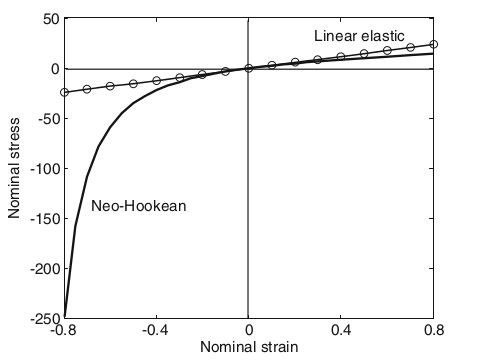
\includegraphics[scale=0.7]{Figure2/Chap3/neohk.png}
    \caption{Stress–strain relationship for Neo–Hookean material in example}
    \label{fig:3.13}
\end{figure}

